\chapter{Discussion}
Please tell more about conclusion and how to the next work of this study.

\section{Andi Muhammad Aslam/1164064}
\subsection{Teori}
\begin{enumerate}
\item Jelaskan kenapa file teks harus di lakukan tokenizer.
\subitem Tahap Tokenizing adalah tahap pemotongan string input berdasarkan tiap kata yang menyusunnya. Tokenisasi secara garis besar memecah sekumpulan karakter dalam suatu teks ke dalam satuan kata, bagaimana membedakan karakter-karakter tertentu yang dapat diperlakukan sebagai pemisah kata atau bukan. Sebagai contoh karakter whitespace, seperti enter, tabulasi, spasi dianggap sebagai pemisah kata. Namun untuk karakter petik tunggal (‘), titik (.), semikolon (;), titk dua (:) atau lainnya, dapat memiliki peran yang cukup banyak sebagai pemisah kata.
\begin{figure}[!htbp]
	\centerline{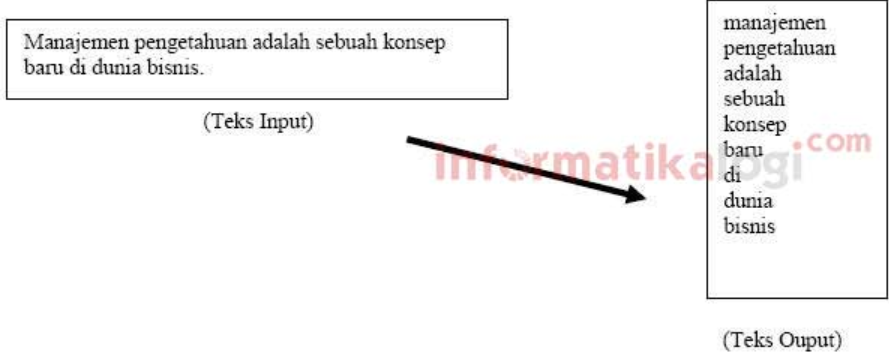
\includegraphics[width=1\textwidth]{figures/andi/7-1.PNG}}
	\caption{Tokenizer}
	\label{Teori}
\end{figure}

\item Jelaskan konsep dasar K Fold Cross Validation pada dataset komentar Youtube pada kode listing 7.1.dilengkapi dengan ilustrasi atau gambar.
\subitem Starfiedkfold yaitu mengembalikan lipatan data bertingkat. Lipatan dibuat dengan mempertahankan presentase sampel setiap kelas dari dataset youtube. dari contoh sampel dalam ilustrasi mempresentasikan sampel dataset menjadi 5 bagian di setiap kelasnya.

\begin{lstlisting}[caption=K Fold Cross Validation,label={lst:7.0}]
kfold = StratifiedKFold(n_splits=5)
splits = kfold.split(d, d['CLASS'])
\end{lstlisting}

\item Berikut ilustrasi pada K Fold Cross Validation :
\begin{figure}[ht]
\centering
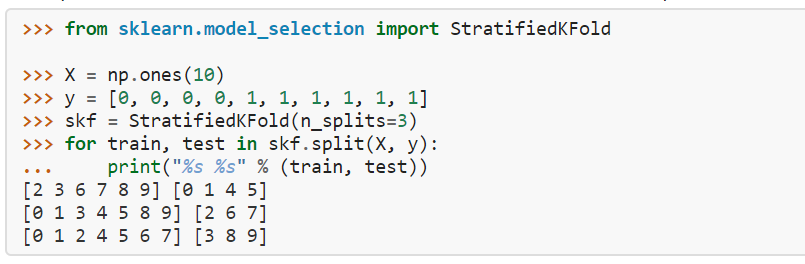
\includegraphics[scale=0.5]{figures/andi/7-2.PNG}
\caption{ KFold Cross validation}
\label{Teori}
\end{figure}

\item Jelaskan apa maksudnya kode program for train, test in splits. dilengkapi denganilustrasi atau gambar.
\subitem Maksudnya For Train, test in split untuk menguji dataset yang sudah di split sebelumnya agar tidak terjadi penumpukkan, yaitu dengan cepat dapat mengelompokkan validasi input data dan dapat di ShuffleSplit dan aplikasi untuk memasukkan data ke dalam satu panggilan tunggal agar dapat memisahkan data secara opsional dan subsampling.

\item Berikut ilustrasi pada for train, test in splits :
\begin{figure}[ht]
\centering
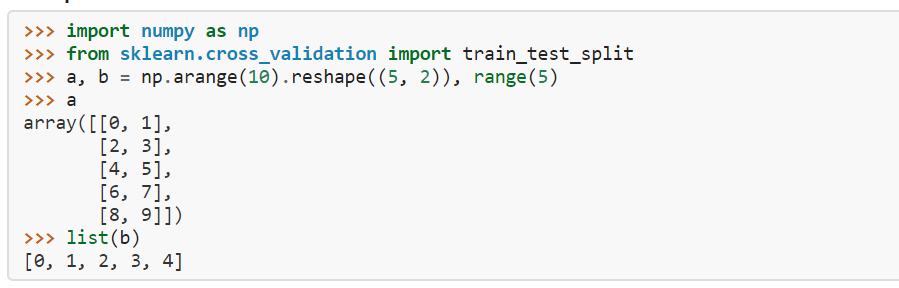
\includegraphics[scale=0.5]{figures/andi/7-3.PNG}
\caption{Ilustrasi for train, test in splits}
\label{Teori}
\end{figure}


\item Jelaskan apa itu Deep Learning.
\subitem Deep Learning adalah salah satu jenis algoritma jaringan saraf tiruan yang menggunakan metadata sebagai input dan mengolahnya menggunakan sejumlah lapisan tersembunyi (hidden layer) transformasi non linier dari data masukan untuk menghitung nilai output. Algortima pada Deep Learning memiliki fitur yang unik yaitu sebuah fitur yang mampu mengekstraksi secara otomatis.
\item Jelaskan apa itu Deep Neural dan bedanya dengan Deep Learning.
\begin{itemize}
\item Deep Neural Network atau DNN merupakan algoritma yang berbasis neural network yang digunakan untuk mengambil keputusan.
\item Yang membedakan Deep Learning dengan  Deep Neural Network (DNN) adalah DNN merupakan algoritma yang digunakan pada Deep Learning, sedangkan Deep Learning merupakan model yang menggunakan algoritma DNN.
\end{itemize}
\end{enumerate}

\section{Aip Suprapto Munari-1164063}
\subsection{Teori}
\begin{enumerate}
\item Kenapa File Suara Harus Dilakukan Tokenizer
\begin{itemize}
\item Penjelasan: Untuk membedakan karakter-karakter tertentu dalam suatu teks dan juga sebagai pemisah kata atau bukan.Tokenizer dilakukan dengan cara melakukan pemotongan string input berdasarkan tiap kata yang menyusunnya.
\par 
\par
\item Ilustrasi Gambar
\item Tokenizer \ref{teori1}
\begin{figure}[!hbtp]
\centering
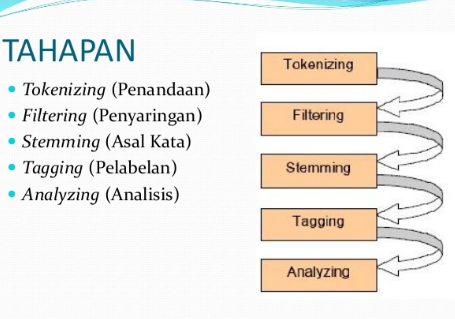
\includegraphics[scale=0.7]{figures/AIP/g1.PNG}
\caption{Tokenizer Aip}
\label{teori1}
\end{figure}
\par
\end{itemize}
\par
\par

\item 	Apa Itu Deep Learning
\begin{itemize}
\item Penjelasan: 
\par  Deep learning merupakan sub bidang pembelajaran mesin yang berkaitan dengan algoritma.
\end{itemize}
\par
\par

\item Apa itu Deep Neural Network Dan Apa Bedanya Dengan Deep Learning :
\begin{itemize}
\item Penjelasan Deep Neural Network : 
\par  Deep neural network adalah jaringan syaraf dengan tingkat kompleksitas tertentu, jaringan syaraf dengan lebih dari dua lapisan.
\par
\item Perbedaan Deep Neural Network Dan Deep Learning :
\par Perbedaan antara deep neural network dan deep learning terletak pada kedalaman model. deep learning adalah frasa yang digunakan untuk jaringan saraf yang kompleks. Kompleksitas ini disebabkan oleh pola yang rumit tentang bagaimana informasi dapat mengalir di seluruh model.
\end{itemize}
\par
\par

\end{enumerate}